% !TEX root = ../OT4ML.tex

%%%%%%%%%%%%%%%%%%%%%%%%%%%%%%%%%%%%%%%%%%%%%%%%%%%%%%%%%%%%%%%%%%%%%%%%%%%
%%%%%%%%%%%%%%%%%%%%%%%%%%%%%%%%%%%%%%%%%%%%%%%%%%%%%%%%%%%%%%%%%%%%%%%%%%%
%%%%%%%%%%%%%%%%%%%%%%%%%%%%%%%%%%%%%%%%%%%%%%%%%%%%%%%%%%%%%%%%%%%%%%%%%%%
\section{Generalized Wasserstein Distances}
\label{sec-extensions}
\label{sec-generalized-wasserstein-distances}

The first family of extensions keeps the idea of a distance between measures, but changes the geometry used to compare them. The variants below relax mass conservation, reduce high-dimensional transport to one-dimensional projections, or replace the trace quadratic cost by spectral gauges and robust projected viewpoints. They are useful when standard $\Wass_p$ is too rigid or too expensive, while still preserving a metric interpretation.

%%%%%%%%%%%%%%%%%%%%%%%%%%%%%%%%%%%%%%%%%%%%%%%%%%%%%%%%%%%%%%%%%%%%%%%%%%%
\subsection{Unbalanced OT}
\label{sec-unbalanced}

Unbalanced OT allows mass creation and destruction by penalizing marginal mismatch. This is essential when histograms are not normalized, when observations contain outliers, or when only part of the source should match the target~\cite{LieroMielkeSavareLong,2015-chizat-unbalanced,2017-chizat-focm}.

%%%
\paragraph{Relaxed formulation.}

For nonnegative measures $(\al,\be) \in \Mm_+(\Xx) \times \Mm_+(\Yy)$, a generic relaxed formulation is
\eql{\label{eq-unbalanced-primal}
	\UW_c(\al,\be)= \uinf{\pi \in \Mm_+(\Xx \times \Yy)} \int_{\Xx \times \Yy} c(x,y) \d\pi(x,y)
		+ \Dd_{\psi_1}(\pi_1|\al) + \Dd_{\psi_2}(\pi_2|\be),
}
where $\psi_1,\psi_2$ are convex entropy functions. Exact conservation $(\pi_1,\pi_2)=(\al,\be)$ is replaced by a cost for changing the marginals. Writing $\psi_s=\tau\bar\psi_s$ exposes the relaxation scale:
\[
	\UW_{c,\tau}(\alpha,\beta)
	=
	\inf_{\pi\geq0}
	\int c\d\pi
	+
	\tau\Dd_{\bar\psi_1}(\pi_1|\alpha)
	+
	\tau\Dd_{\bar\psi_2}(\pi_2|\beta).
\]
Large $\tau$ makes marginal mismatch expensive and approaches balanced OT when the total masses are compatible. Small $\tau$ makes it cheaper to destroy source mass and create target mass instead of transporting it over long distances.

%%%
\paragraph{Homogeneous viewpoint.}

The conic formulation of unbalanced OT is obtained by rewriting the marginal penalties as a local cost. For positive density ratios $r,s$, set
\eql{\label{eq-unbalanced-reverse-local-cost}
	L_c(r,s) \eqdef c + r\psi_1(1/r)+s\psi_2(1/s).
}
Its positively homogeneous perspective is
\eql{\label{eq-unbalanced-homogeneous-local-cost}
	H_c(r,s) \eqdef \inf_{\theta>0} \theta L_c(r/\theta,s/\theta).
}
The associated homogeneous unbalanced value can be written formally as
\eql{\label{eq-homogeneous}
	\HW_c(\al,\be)
	=
	\inf_{\pi\geq0}
	\int H_{c(x,y)}\!\left(\frac{\d\pi_1}{\d\al}(x),\frac{\d\pi_2}{\d\be}(y)\right)\d\pi(x,y),
}
with the usual recession terms on the singular parts. This perspective is the right one for proving metric properties.

\begin{thm}[Cone formulation of unbalanced OT]\label{thm-cone-unbalanced-ot}
	Assume $\Xx=\Yy$, $\psi_1=\psi_2$, and choose the ground cost and exponent so that
	\[
		\De((x,r),(y,s)) \eqdef H_{c(x,y)}(r^p,s^p)^{1/p}
	\]
	is a distance on the cone $\mathfrak C[\Xx]$. Then $\UW_c=\HW_c$ and the corresponding cone OT value $\CW_c^{1/p}$ is a distance between nonnegative measures.
\end{thm}

\begin{proof}
	The equality $\UW_c=\HW_c$ follows from the perspective relaxation: disintegrating a feasible plan with respect to its marginals turns the marginal penalties into the local expression $L_c$, and optimizing over a common scaling variable gives $H_c$ without changing the infimum. Lifting each point $x$ to a cone point $(x,r)$ encodes the transported amount as the radial coordinate. The cone marginal constraints recover $\al$ and $\be$ after integrating $r^p$ and $s^p$. If $\De$ is a distance, the cone formulation is ordinary Wasserstein transport on a metric cone, hence its $p$th root satisfies symmetry, separation and the triangle inequality.
\end{proof}

%%%
\paragraph{Entropic KL relaxation.}

For discrete histograms $\a,\b$ and a cost matrix $\C$, the KL-penalized entropic problem reads
\[
	\min_{\P\geq0}
	\dotp{\C}{\P}
	+\epsilon\KL(\P|\a\otimes\b)
	+\tau\KL(\P\ones|\a)
	+\tau\KL(\transp{\P}\ones|\b).
\]
With $K_{i,j}=e^{-\C_{i,j}/\epsilon}\a_i\b_j$ and $\rho=\tau/(\tau+\epsilon)$, the generalized Sinkhorn scaling is
\[
	u_i\leftarrow \left(\frac{\a_i}{(K v)_i}\right)^\rho,
	\qquad
	v_j\leftarrow \left(\frac{\b_j}{(\transp{K}u)_j}\right)^\rho,
	\qquad
	\P=\diag(u)K\diag(v).
\]
The exponent $\rho<1$ is the visible difference with balanced Sinkhorn: marginal corrections are damped because violating the marginals is allowed.

\begin{figure}[H]
\centering
\setlength{\tabcolsep}{3pt}
\begin{tabular}{@{}ccc@{}}
\small small $\tau$ & \small medium $\tau$ & \small large $\tau$ \\[-.15em]

\includegraphics[width=.30\linewidth]{figures/unbalanced-mass-relaxation/tau-small.pdf} &

\includegraphics[width=.30\linewidth]{figures/unbalanced-mass-relaxation/tau-medium.pdf} &

\includegraphics[width=.30\linewidth]{figures/unbalanced-mass-relaxation/tau-large.pdf}
\end{tabular}
\caption{KL unbalanced OT on one-dimensional Gaussian-mixture densities. The central matrix is the transported coupling. On the left, the red curve is the prescribed source marginal and the violet curve is the transported source marginal; the red gap is destroyed mass. On the top, the blue curve is the prescribed target marginal and the violet curve is the transported target marginal; the blue gap is created mass. Increasing $\tau$ makes marginal mismatch more expensive, so more mass is transported, including toward the far right target mode.}
\label{fig:unbalanced-mass-relaxation}
\end{figure}

The entropy used in the marginal relaxation also changes the qualitative behavior. A KL penalty leads to smooth multiplicative rescaling. The reverse-KL, or Burg, penalty blows up when a transported marginal vanishes where the prescribed marginal is positive, so it discourages complete deletion of small modes. Total variation has a linear kink and behaves closer to partial transport: mass is either kept active or created and destroyed at nearly constant marginal price.

\begin{figure}[H]
\centering
\setlength{\tabcolsep}{3pt}
\begin{tabular}{@{}ccc@{}}
\small KL & \small Burg & \small total variation \\[-.15em]

\includegraphics[width=.30\linewidth]{figures/unbalanced-divergence-choice/kl.pdf} &

\includegraphics[width=.30\linewidth]{figures/unbalanced-divergence-choice/burg.pdf} &

\includegraphics[width=.30\linewidth]{figures/unbalanced-divergence-choice/tv.pdf}
\end{tabular}
\caption{Effect of the marginal divergence in unbalanced entropic OT. The geometric cost, entropic plan regularization $\epsilon$, and relaxation strength $\tau$ are fixed; only the marginal penalty changes. KL allows smooth mass variation, Burg keeps transported marginals from vanishing on prescribed modes, and total variation gives a sharper active-mass selection. The side plots use the same convention as Figure~\ref{fig:unbalanced-mass-relaxation}.}
\label{fig:unbalanced-divergence-choice}
\end{figure}

%%%%%%%%%%%%%%%%%%%%%%%%%%%%%%%%%%%%%%%%%%%%%%%%%%%%%%%%%%%%%%%%%%%%%%%%%%%
\subsection{Sliced Wasserstein Distances}
\label{sec-sliced-wasserstein}

Sliced Wasserstein replaces one hard high-dimensional OT problem by many one-dimensional OT problems. For $\theta\in\Sphere^{d-1}$, let $P_\theta(x)=\dotp{\theta}{x}$ be the projection on direction $\theta$. The sliced distance is
\eql{\label{eq-sliced-wasserstein}
	\SW_p(\al,\be)^p
	\eqdef
	\int_{\Sphere^{d-1}}
	\Wass_p\big((P_\theta)_\sharp\al,(P_\theta)_\sharp\be\big)^p
	\d\sigma(\theta),
}
where $\sigma$ is the uniform probability measure on the sphere. This construction is computationally attractive because each projected problem is solved by sorting or quantiles~\cite{rabin-ssvm-11,2013-Bonneel-barycenter,kolouri2016sliced}.

\begin{figure}[H]
\centering
\setlength{\tabcolsep}{3pt}
\begin{tabular}{@{}cccc@{}}
\small source density & \small source slices & \small target slices & \small target density \\[-.15em]
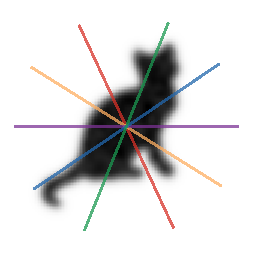
\includegraphics[width=.23\linewidth]{figures/sliced-wasserstein-projections/density-alpha.pdf} &
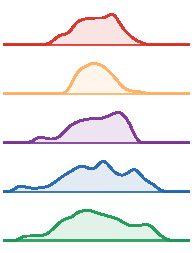
\includegraphics[width=.17\linewidth]{figures/sliced-wasserstein-projections/hist-alpha.pdf} &

\includegraphics[width=.17\linewidth]{figures/sliced-wasserstein-projections/hist-beta.pdf} &

\includegraphics[width=.23\linewidth]{figures/sliced-wasserstein-projections/density-beta.pdf}
\end{tabular}
\caption{Sliced Wasserstein projections between two planar densities. Five fixed directions are drawn on the source and target point clouds. For each direction, the middle panels show the one-dimensional projected histograms $(P_\theta)_\sharp\alpha$ and $(P_\theta)_\sharp\beta$. Sliced OT averages one-dimensional Wasserstein discrepancies over many such directions, replacing a difficult planar comparison by a collection of sorted one-dimensional comparisons.}
\label{fig:sliced-wasserstein-projections}
\end{figure}

\begin{defn}[Sliced variants]\label{def-sliced-variants}
	The max-sliced distance replaces the average in~\eqref{eq-sliced-wasserstein} by a supremum,
	\[
		\MaxSW_p(\al,\be)^p
		\eqdef
		\sup_{\theta\in\Sphere^{d-1}}
		\Wass_p\big((P_\theta)_\sharp\al,(P_\theta)_\sharp\be\big)^p.
	\]
	The same definitions can be made with projections on $k$-dimensional subspaces, giving $\SW_{p,k}$ and $\MaxSW_{p,k}$. Min-sliced lifted plans keep the projection direction but lift the induced one-dimensional matching back to the ambient space, giving an interpretable upper-bound construction for $\Wass_2$.
\end{defn}

\begin{figure}[H]
\centering
\setlength{\tabcolsep}{3pt}
\begin{tabular}{@{}ccc@{}}
\small selected projection & \small lifted sliced plan & \small quadratic $W_2$ plan \\[-.15em]

\includegraphics[width=.30\linewidth]{figures/min-sliced-transport-plan/direction.pdf} &
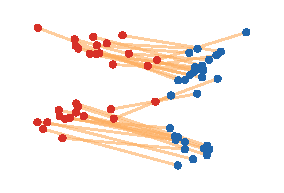
\includegraphics[width=.30\linewidth]{figures/min-sliced-transport-plan/lifted-plan.pdf} &

\includegraphics[width=.30\linewidth]{figures/min-sliced-transport-plan/w2-plan.pdf}
\end{tabular}
\caption{Lifted min-sliced plan. A one-dimensional direction is selected by a small deterministic sweep, then red and blue atoms are sorted after projection and matched in that order. The middle panel lifts this one-dimensional matching back to the plane; it is a feasible coupling but not the same object as the quadratic $W_2$ matching shown on the right. This illustrates why sliced constructions are computationally light and interpretable, while losing some of the geometry of the full transport problem.}
\label{fig:min-sliced-transport-plan}
\end{figure}

%%%%%%%%%%%%%%%%%%%%%%%%%%%%%%%%%%%%%%%%%%%%%%%%%%%%%%%%%%%%%%%%%%%%%%%%%%%
\subsection{Spectral and Robust Wasserstein Distances}
\label{sec-spectral-subspace-wasserstein}

For quadratic cost, an OT coupling has a second-moment displacement matrix
\[
	M_\pi \eqdef \int (x-y)(x-y)^\top \d\pi(x,y) \in \mathbb S_+^d.
\]
Standard $\Wass_2^2$ corresponds to the trace gauge $M\mapsto\tr(M)$. More generally, let $\gamma:\mathbb S_+^d\to\RR_+$ be a monotone gauge, meaning that it is convex, positively homogeneous, vanishes only at $0$, and is monotone for the Loewner order: $0\preceq M\preceq N$ implies $\gamma(M)\leq\gamma(N)$. Define
\eql{\label{eq-spectral-wasserstein}
	\Wass_\gamma(\al,\be)^2
	\eqdef
	\inf_{\pi\in\Couplings(\al,\be)} \gamma(M_\pi).
}
The trace gauge gives back $\Wass_2$. The spectral gauge $\gamma(M)=\lambda_{\max}(M)$ instead measures the worst transported variance direction.

The polar set of the gauge is
\eql{\label{eq-spectral-polar-set}
	\mathcal B_\gamma
	\eqdef
	\enscond{A\succeq0}{\dotp{A}{M}\leq\gamma(M)\quad\text{for all }M\succeq0},
}
so that $\gamma(M)=\sup_{A\in\mathcal B_\gamma}\dotp{A}{M}$. For $A\succeq0$, introduce the projected quadratic transport cost
\eql{\label{eq-quadratic-projected-cost}
	\Wass_{2,A}(\al,\be)^2
	\eqdef
	\inf_{\pi\in\Couplings(\al,\be)}
	\int \dotp{A}{(x-y)(x-y)^\top}\d\pi(x,y).
}

\begin{prop}[Robust form of spectral Wasserstein]
	Assume the measures have compact support and $\mathcal B_\gamma$ is compact. Then
	\[
		\Wass_\gamma(\al,\be)
		=
		\sup_{A\in\mathcal B_\gamma} \Wass_{2,A}(\al,\be).
	\]
	In particular, if $a\tr(M)\leq\gamma(M)\leq b\tr(M)$ on $\mathbb S_+^d$ for some $0<a\leq b<\infty$, then $\Wass_\gamma$ is a distance and is equivalent to $\Wass_2$.
\end{prop}

\begin{proof}
	Using the support-function representation of $\gamma$,
	\[
		\Wass_\gamma(\al,\be)^2
		=
		\inf_{\pi\in\Couplings(\al,\be)}\sup_{A\in\mathcal B_\gamma}
		\int \dotp{A}{(x-y)(x-y)^\top}\d\pi.
	\]
	The coupling set is compact and convex for compactly supported measures, $\mathcal B_\gamma$ is compact and convex, and the displayed functional is bilinear in $(\pi,A)$. Sion's minimax theorem exchanges the infimum and supremum and gives the robust formula. Each $\Wass_{2,A}$ is a pseudometric, so the supremum is a metric as soon as the polar family detects every nonzero displacement. The two trace bounds give
	\[
		\sqrt a\,\Wass_2(\al,\be)
		\leq
		\Wass_\gamma(\al,\be)
		\leq
		\sqrt b\,\Wass_2(\al,\be),
	\]
	which proves separation and equivalence.
\end{proof}

The Paty--Cuturi subspace robust distance~\cite{paty2019subspace} is recovered by choosing the polar family $\mathcal B$ to be rank-$k$ orthogonal projectors. Its convex hull is $\enscond{A}{0\preceq A\preceq I,\ \tr(A)=k}$, and the associated support function is the Ky Fan gauge $\gamma_k$. Thus $\Wass_{\gamma_k}$ is the convexified spectral counterpart of $\SRW_{2,k}$, while $\SRW_{2,k}$ keeps the original non-convex rank constraint. For $k=1$, $\gamma_1(M)=\lambda_{\max}(M)$ and $\mathcal B_{\gamma_1}=\enscond{A\succeq0}{\tr(A)\leq1}$. This top-eigenvalue spectral Wasserstein geometry is connected to Muon-type spectral dynamics in~\cite{peyre2026muon}.

\begin{figure}[H]
\centering
\setlength{\tabcolsep}{3pt}
\begin{tabular}{@{}cc@{}}
\small trace-gauge coupling & \small $\lambda_{\max}$-gauge coupling \\[-.15em]

\includegraphics[width=.36\linewidth]{figures/spectral-wasserstein-gauge/trace-coupling.pdf} &

\includegraphics[width=.36\linewidth]{figures/spectral-wasserstein-gauge/lambda-max-coupling.pdf}
\\[-.1em]
\small trace-gauge interpolation & \small $\lambda_{\max}$-gauge interpolation \\[-.15em]

\includegraphics[width=.36\linewidth]{figures/spectral-wasserstein-gauge/trace-geodesic.pdf} &

\includegraphics[width=.36\linewidth]{figures/spectral-wasserstein-gauge/lambda-max-geodesic.pdf}
\end{tabular}
\caption{Trace and spectral gauges for displacement covariances. The trace gauge minimizes the average squared displacement and gives the usual quadratic transport plan. The $\lambda_{\max}$ gauge penalizes the worst projected displacement variance; the displayed plan is obtained by a small finite-direction robust linear program. The bottom row shows the corresponding displacement interpolations, colored from red to blue. The figure is illustrative: it visualizes how changing the gauge changes the coupling and the induced interpolation geometry.}
\label{fig:spectral-wasserstein-gauge}
\end{figure}

%%%%%%%%%%%%%%%%%%%%%%%%%%%%%%%%%%%%%%%%%%%%%%%%%%%%%%%%%%%%%%%%%%%%%%%%%%%
%%%%%%%%%%%%%%%%%%%%%%%%%%%%%%%%%%%%%%%%%%%%%%%%%%%%%%%%%%%%%%%%%%%%%%%%%%%
%%%%%%%%%%%%%%%%%%%%%%%%%%%%%%%%%%%%%%%%%%%%%%%%%%%%%%%%%%%%%%%%%%%%%%%%%%%
